% Options for packages loaded elsewhere
\PassOptionsToPackage{unicode}{hyperref}
\PassOptionsToPackage{hyphens}{url}
%
\documentclass[
  ignorenonframetext,
]{beamer}
\usepackage{pgfpages}
\setbeamertemplate{caption}[numbered]
\setbeamertemplate{caption label separator}{: }
\setbeamercolor{caption name}{fg=normal text.fg}
\beamertemplatenavigationsymbolsempty
% Prevent slide breaks in the middle of a paragraph
\widowpenalties 1 10000
\raggedbottom
\setbeamertemplate{part page}{
  \centering
  \begin{beamercolorbox}[sep=16pt,center]{part title}
    \usebeamerfont{part title}\insertpart\par
  \end{beamercolorbox}
}
\setbeamertemplate{section page}{
  \centering
  \begin{beamercolorbox}[sep=12pt,center]{part title}
    \usebeamerfont{section title}\insertsection\par
  \end{beamercolorbox}
}
\setbeamertemplate{subsection page}{
  \centering
  \begin{beamercolorbox}[sep=8pt,center]{part title}
    \usebeamerfont{subsection title}\insertsubsection\par
  \end{beamercolorbox}
}
\AtBeginPart{
  \frame{\partpage}
}
\AtBeginSection{
  \ifbibliography
  \else
    \frame{\sectionpage}
  \fi
}
\AtBeginSubsection{
  \frame{\subsectionpage}
}
\usepackage{lmodern}
\usepackage{amsmath}
\usepackage{ifxetex,ifluatex}
\ifnum 0\ifxetex 1\fi\ifluatex 1\fi=0 % if pdftex
  \usepackage[T1]{fontenc}
  \usepackage[utf8]{inputenc}
  \usepackage{textcomp} % provide euro and other symbols
  \usepackage{amssymb}
\else % if luatex or xetex
  \usepackage{unicode-math}
  \defaultfontfeatures{Scale=MatchLowercase}
  \defaultfontfeatures[\rmfamily]{Ligatures=TeX,Scale=1}
\fi
% Use upquote if available, for straight quotes in verbatim environments
\IfFileExists{upquote.sty}{\usepackage{upquote}}{}
\IfFileExists{microtype.sty}{% use microtype if available
  \usepackage[]{microtype}
  \UseMicrotypeSet[protrusion]{basicmath} % disable protrusion for tt fonts
}{}
\makeatletter
\@ifundefined{KOMAClassName}{% if non-KOMA class
  \IfFileExists{parskip.sty}{%
    \usepackage{parskip}
  }{% else
    \setlength{\parindent}{0pt}
    \setlength{\parskip}{6pt plus 2pt minus 1pt}}
}{% if KOMA class
  \KOMAoptions{parskip=half}}
\makeatother
\usepackage{xcolor}
\IfFileExists{xurl.sty}{\usepackage{xurl}}{} % add URL line breaks if available
\IfFileExists{bookmark.sty}{\usepackage{bookmark}}{\usepackage{hyperref}}
\hypersetup{
  pdftitle={Making Migration Sexy: How State and National Policies Influence Migration of Same-Sex Couples},
  hidelinks,
  pdfcreator={LaTeX via pandoc}}
\urlstyle{same} % disable monospaced font for URLs
\newif\ifbibliography
\usepackage{graphicx}
\makeatletter
\def\maxwidth{\ifdim\Gin@nat@width>\linewidth\linewidth\else\Gin@nat@width\fi}
\def\maxheight{\ifdim\Gin@nat@height>\textheight\textheight\else\Gin@nat@height\fi}
\makeatother
% Scale images if necessary, so that they will not overflow the page
% margins by default, and it is still possible to overwrite the defaults
% using explicit options in \includegraphics[width, height, ...]{}
\setkeys{Gin}{width=\maxwidth,height=\maxheight,keepaspectratio}
% Set default figure placement to htbp
\makeatletter
\def\fps@figure{htbp}
\makeatother
\setlength{\emergencystretch}{3em} % prevent overfull lines
\providecommand{\tightlist}{%
  \setlength{\itemsep}{0pt}\setlength{\parskip}{0pt}}
\setcounter{secnumdepth}{-\maxdimen} % remove section numbering
\usetheme{Madrid}
\useoutertheme{miniframes} % Alternatively: miniframes, infolines, split
\useinnertheme{circles}
\definecolor{uclablue}{RGB}{39, 116, 174}
\usecolortheme[named=uclablue]{structure}
\usepackage{graphicx}
\usepackage{tikz}
\usepackage{multimedia}
\usepackage[overlay]{textpos}
\usepackage{enumerate}
\usepackage{booktabs}
\usepackage{makecell}
\usepackage{multicol}
\newcommand{\btwocol}{\begin{multicols}{2}}
\newcommand{\etwocol}{\end{multicols}}
\setbeamercovered{transparent}
\DeclareUnicodeCharacter{2212}{-}


%% Notes
%    \setbeameroption{show notes}   
%    \usepackage{pgfpages}
%    \setbeameroption{show notes on second screen}

\AtBeginDocument{\title[Making Migration Sexy]{Making Migration Sexy: How State and National Policies Influence Migration of Same-Sex Couples}}
\AtBeginDocument{\author[Hoffmann \& Velasco]{ Nathan I. Hoffmann, Sociology, UCLA
  \\ Kristopher Velasco, Sociology, UT Austin}}
  

% Defines the graphic but does not place it. See below for that
\titlegraphic{
\includegraphics[width=0.4\paperwidth]{ucla.png}
\includegraphics[width=0.4\paperwidth]{Horizontal-PRC-Logo.png}}

% Creates background bruin bear
\usebackgroundtemplate{%
\tikz[overlay,remember picture] \node[opacity=0.1, at=(current page.south east),anchor=south east]{
\includegraphics[height=0.4\paperheight]{ucla1.png}};}


% Creates the title page I want it to with UCLA logo adjusted
\setbeamertemplate{title page}{%
  \vbox{}
  \vfill
  \begingroup
    \centering
    \begin{beamercolorbox}[sep=8pt,center,colsep=-4bp,rounded=true,shadow=true]{title}
      \usebeamerfont{title}\inserttitle\par%
      \ifx\insertsubtitle\@empty%
      \else%
        \vskip0.25em%
        {\usebeamerfont{subtitle}\usebeamercolor[fg]{subtitle}\insertsubtitle\par}%
      \fi%     
    \end{beamercolorbox}%
    \vskip1em\par
	\insertauthor
	\par
	\insertinstitute
	\vskip2em\par
    {\usebeamercolor[fg]{titlegraphic}\inserttitlegraphic\par}
  \endgroup
  \vfill
}

% Allows me to use two columns
\def\begincols{\begin{columns}}
\def\begincol{\begin{column}}
\def\endcol{\end{column}}
\def\endcols{\end{columns}}



\AtBeginPart{}
\AtBeginSection{}
\AtBeginSubsection{}
\AtBeginSubsubsection{}
\setlength{\emergencystretch}{0em}
\setlength{\parskip}{0pt}
\ifluatex
  \usepackage{selnolig}  % disable illegal ligatures
\fi

\title{Making Migration Sexy: How State and National Policies Influence
Migration of Same-Sex Couples}
\subtitle{PAA 2021 Annual Meeting}
\author{Nathan I. Hoffmann, Department of Sociology, UCLA\\
Kristopher Velasco, Depatment of Sociology, UT Austin}
\date{}

\begin{document}
\frame{\titlepage}

\hypertarget{introduction}{%
\section{Introduction}\label{introduction}}

\begin{frame}{Introduction}
\protect\hypertarget{introduction-1}{}
\begin{itemize}
\tightlist
\item
  2013 Supreme Court struck down DOMA
\item
  From 2013 to 2019, 76\% increase in immigrant same-sex couples,
  compared to 13\% for different-sex
\item
  How has changing policy environment, both at country of origin and in
  U.S. states, contributed toward growth in immigrants in same-sex
  couples?
\item
  How can understanding LGB migration help us better understand the
  links between migration, policy, and identity more broadly?
\end{itemize}
\end{frame}

\begin{frame}{Introduction}
\protect\hypertarget{introduction-2}{}
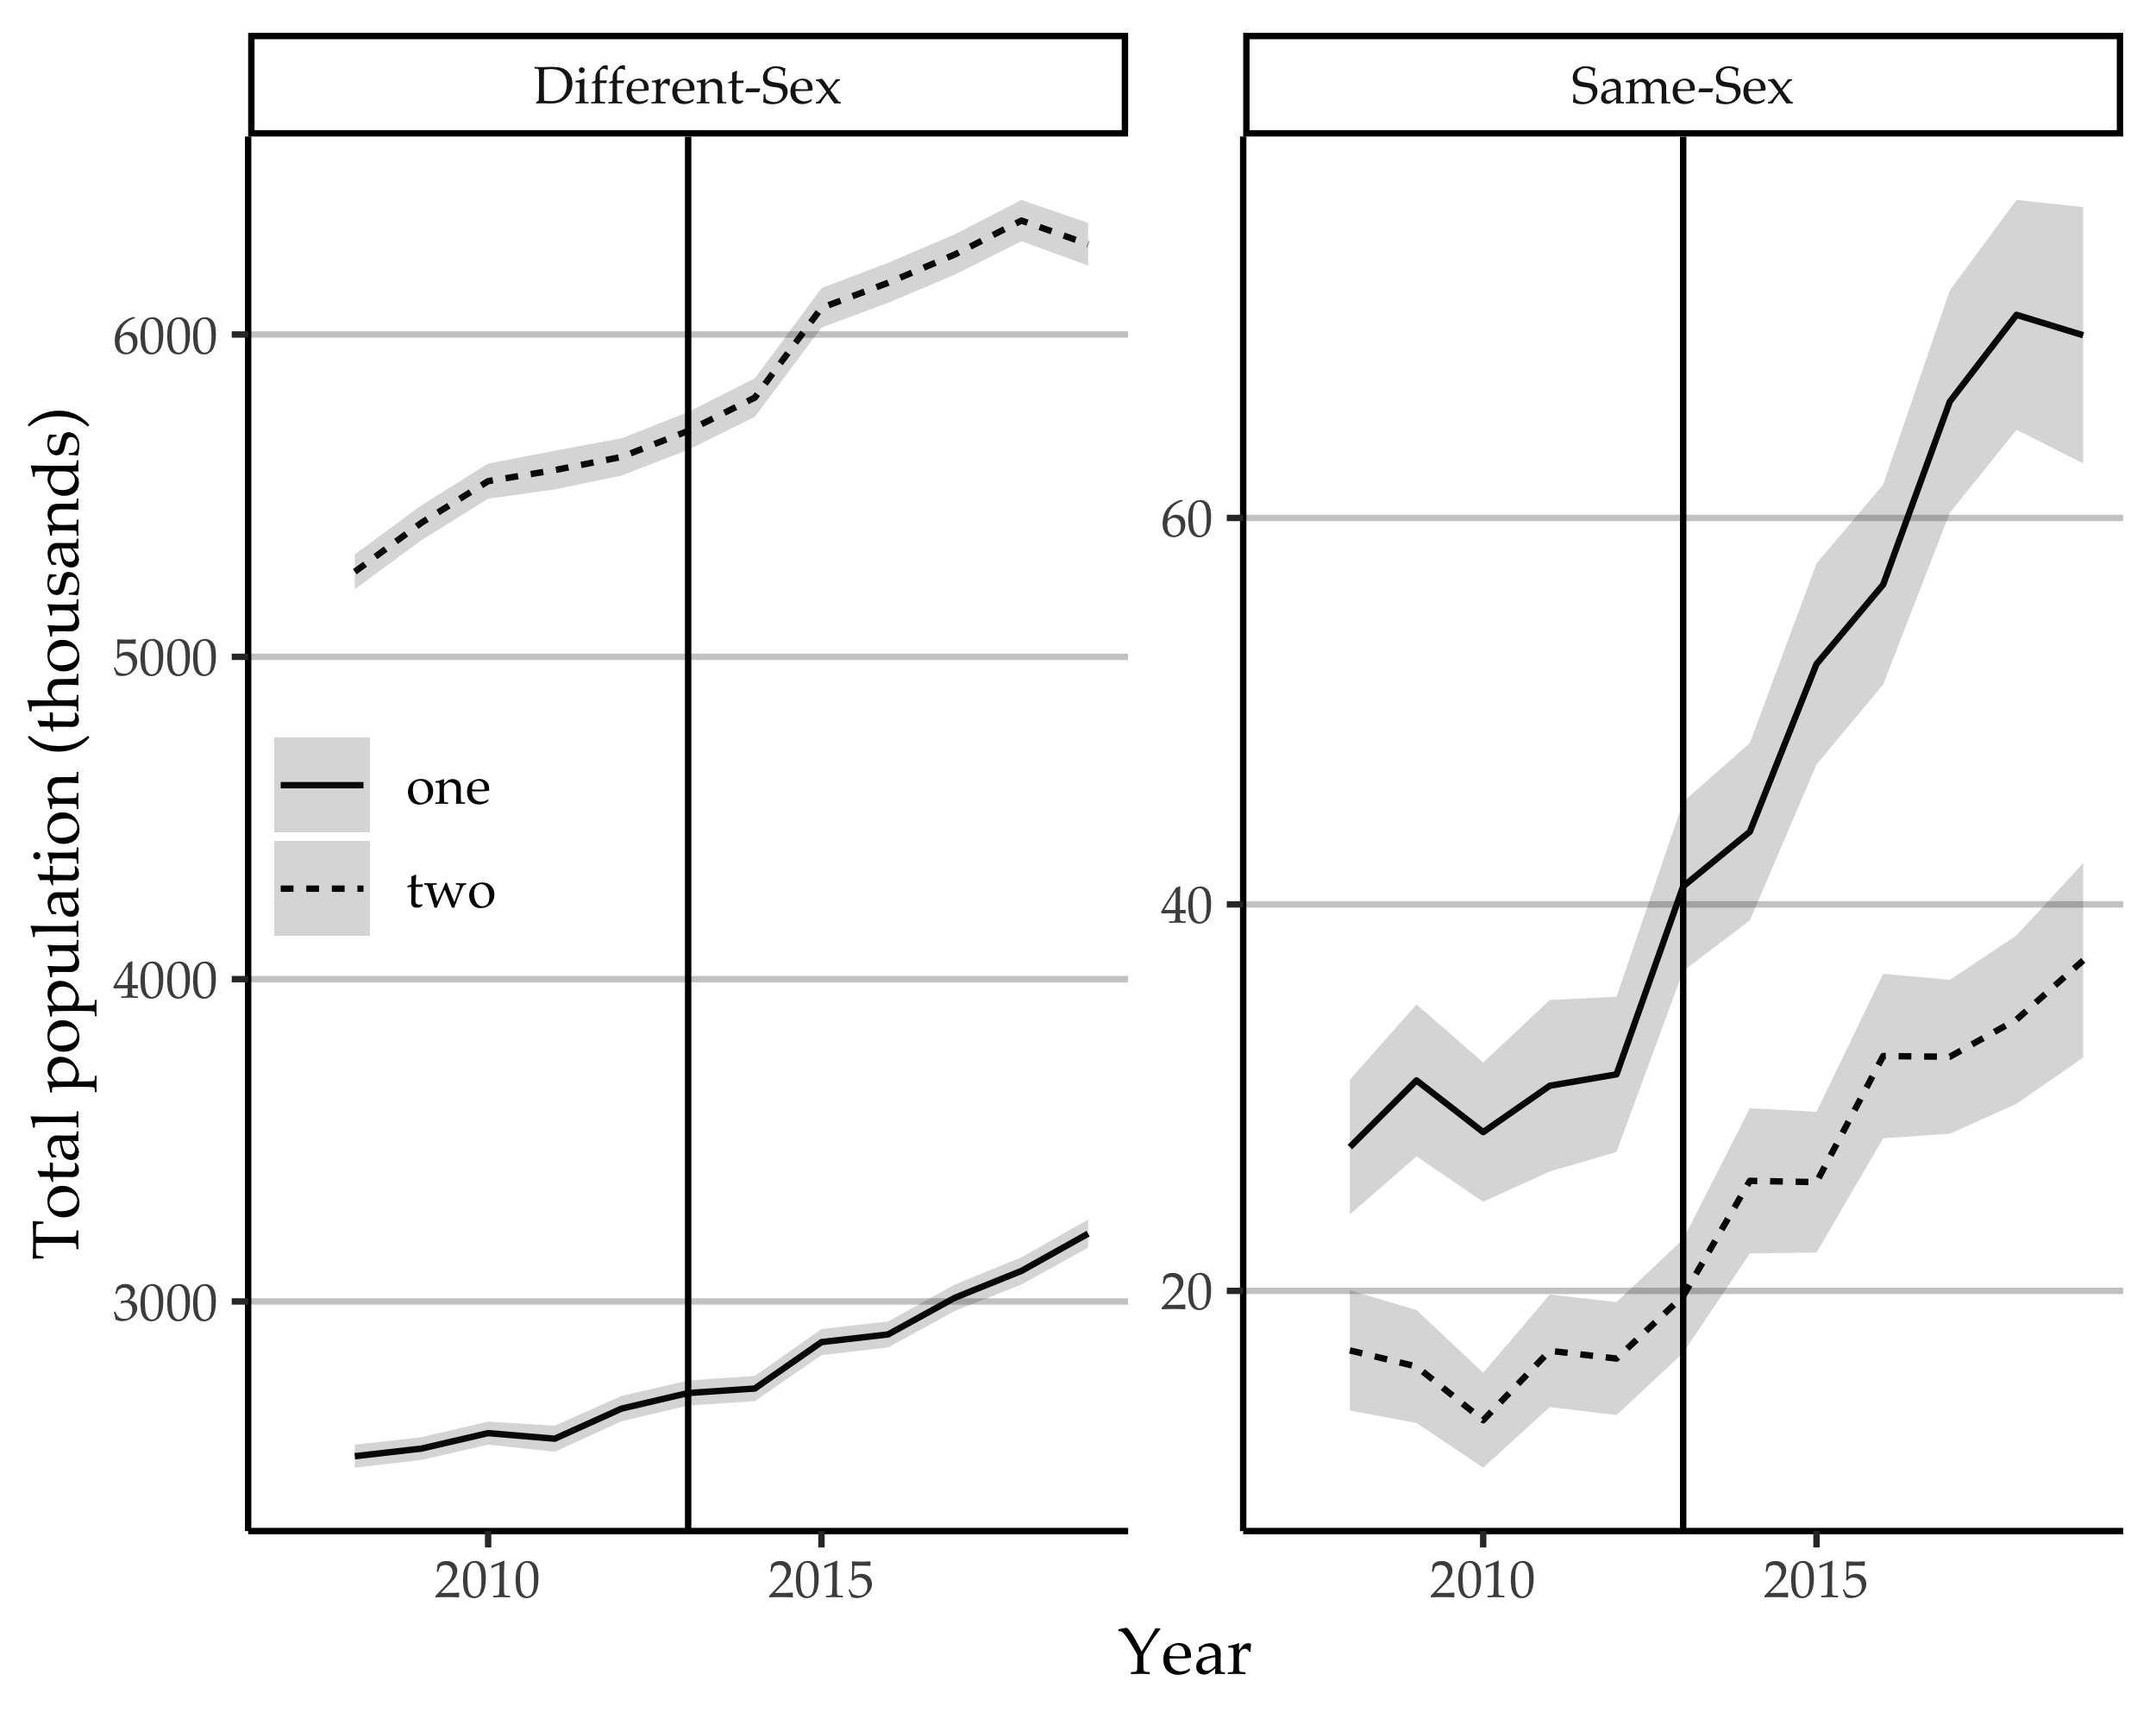
\includegraphics{ssimm_pres_files/figure-beamer/total-pop-1.pdf}
\end{frame}

\hypertarget{background}{%
\section{Background}\label{background}}

\begin{frame}{Conventional Explanations}
\protect\hypertarget{conventional-explanations}{}
\begin{itemize}
\tightlist
\item
  Migration theory relies heavily on economic and network theories
\item
  Recently, culture and social policy considered
\item
  Little previous research applying migration theories to same-sex
  couples. Do they hold up?
\end{itemize}
\end{frame}

\begin{frame}{Our Intervention}
\protect\hypertarget{our-intervention}{}
\begin{itemize}
\tightlist
\item
  We argue that it is imperative to take sexuality, and the state's role
  in governing sexuality, into account for understanding migratory
  patterns
\item
  This population is particularly sensitive to changing policy

  \begin{itemize}
  \tightlist
  \item
    Same-sex relationships were not recognized by the U.S. government
    before the 2013 DOMA decision
  \item
    Policy may overpower traditional migration theories
  \end{itemize}
\end{itemize}
\end{frame}

\begin{frame}{Our Intervention}
\protect\hypertarget{our-intervention-1}{}
\begin{itemize}
\tightlist
\item
  We consider policy at both country of origin and U.S. state
\item
  Country of origin

  \begin{itemize}
  \tightlist
  \item
    Do LGB people choose to flee repressive policy contexts?
  \item
    Or does progressive policy create the capacity for migration?
  \end{itemize}
\item
  U.S. state

  \begin{itemize}
  \tightlist
  \item
    Do immigrants in same-sex couples, like their U.S.-born
    counterparts, choose to live in more progressive states?
  \end{itemize}
\end{itemize}
\end{frame}

\hypertarget{data}{%
\section{Data}\label{data}}

\begin{frame}{Identifying Same-Sex Couples in the ACS}
\protect\hypertarget{identifying-same-sex-couples-in-the-acs}{}
\begin{itemize}
\tightlist
\item
  2008 to 2019 American Community Survey (ACS)

  \begin{itemize}
  \tightlist
  \item
    immigrated at age 18 or older post-1990
  \end{itemize}
\item
  Immigrants in same-sex couples are identified as foreign-born
  respondents who live with a same-sex married or unmarried partner

  \begin{itemize}
  \tightlist
  \item
    This necessarily excludes single and non-cohabiting LGB individuals
  \end{itemize}
\item
  Sample of 7,500 immigrants in same-sex couples compared to 947,227
  immigrants in different-sex couples
\end{itemize}
\end{frame}

\begin{frame}{Variables}
\protect\hypertarget{variables}{}
\begin{itemize}
\tightlist
\item
  Explanatory variables

  \begin{itemize}
  \tightlist
  \item
    Country of origin LGBT policy index (sum of 14 policies)
  \item
    U.S. state LGBT policy index (sum of 8 policies)
  \end{itemize}
\item
  Controls

  \begin{itemize}
  \tightlist
  \item
    Factors from standard migration models, including country- and
    state-level economic, political, and demographic variables from the
    UN, U.S. government, and other sources
  \item
    Individual sociodemographic variables from ACS
  \end{itemize}
\end{itemize}
\end{frame}

\hypertarget{methods}{%
\section{Methods}\label{methods}}

\begin{frame}{Methods}
\protect\hypertarget{methods-1}{}
\begin{itemize}
\tightlist
\item
  \textbf{Analysis 1}: Country-level percentage of immigrants in
  same-sex couples, by country and year of immigration

  \begin{itemize}
  \tightlist
  \item
    OLS regression with country fixed effects
  \end{itemize}
\item
  \textbf{Analysis 2}: State-level percentage of immigrants in same-sex
  couples, by country and year of immigration

  \begin{itemize}
  \tightlist
  \item
    OLS regression with state and country fixed effects
  \end{itemize}
\item
  \textbf{Analysis 3}: Individual-level models predicting state policy
  environment

  \begin{itemize}
  \tightlist
  \item
    Ordered logistic regression with survey-year fixed effects
  \end{itemize}
\end{itemize}
\end{frame}

\hypertarget{results}{%
\section{Results}\label{results}}

\begin{frame}{Descriptive statistics}
\protect\hypertarget{descriptive-statistics}{}
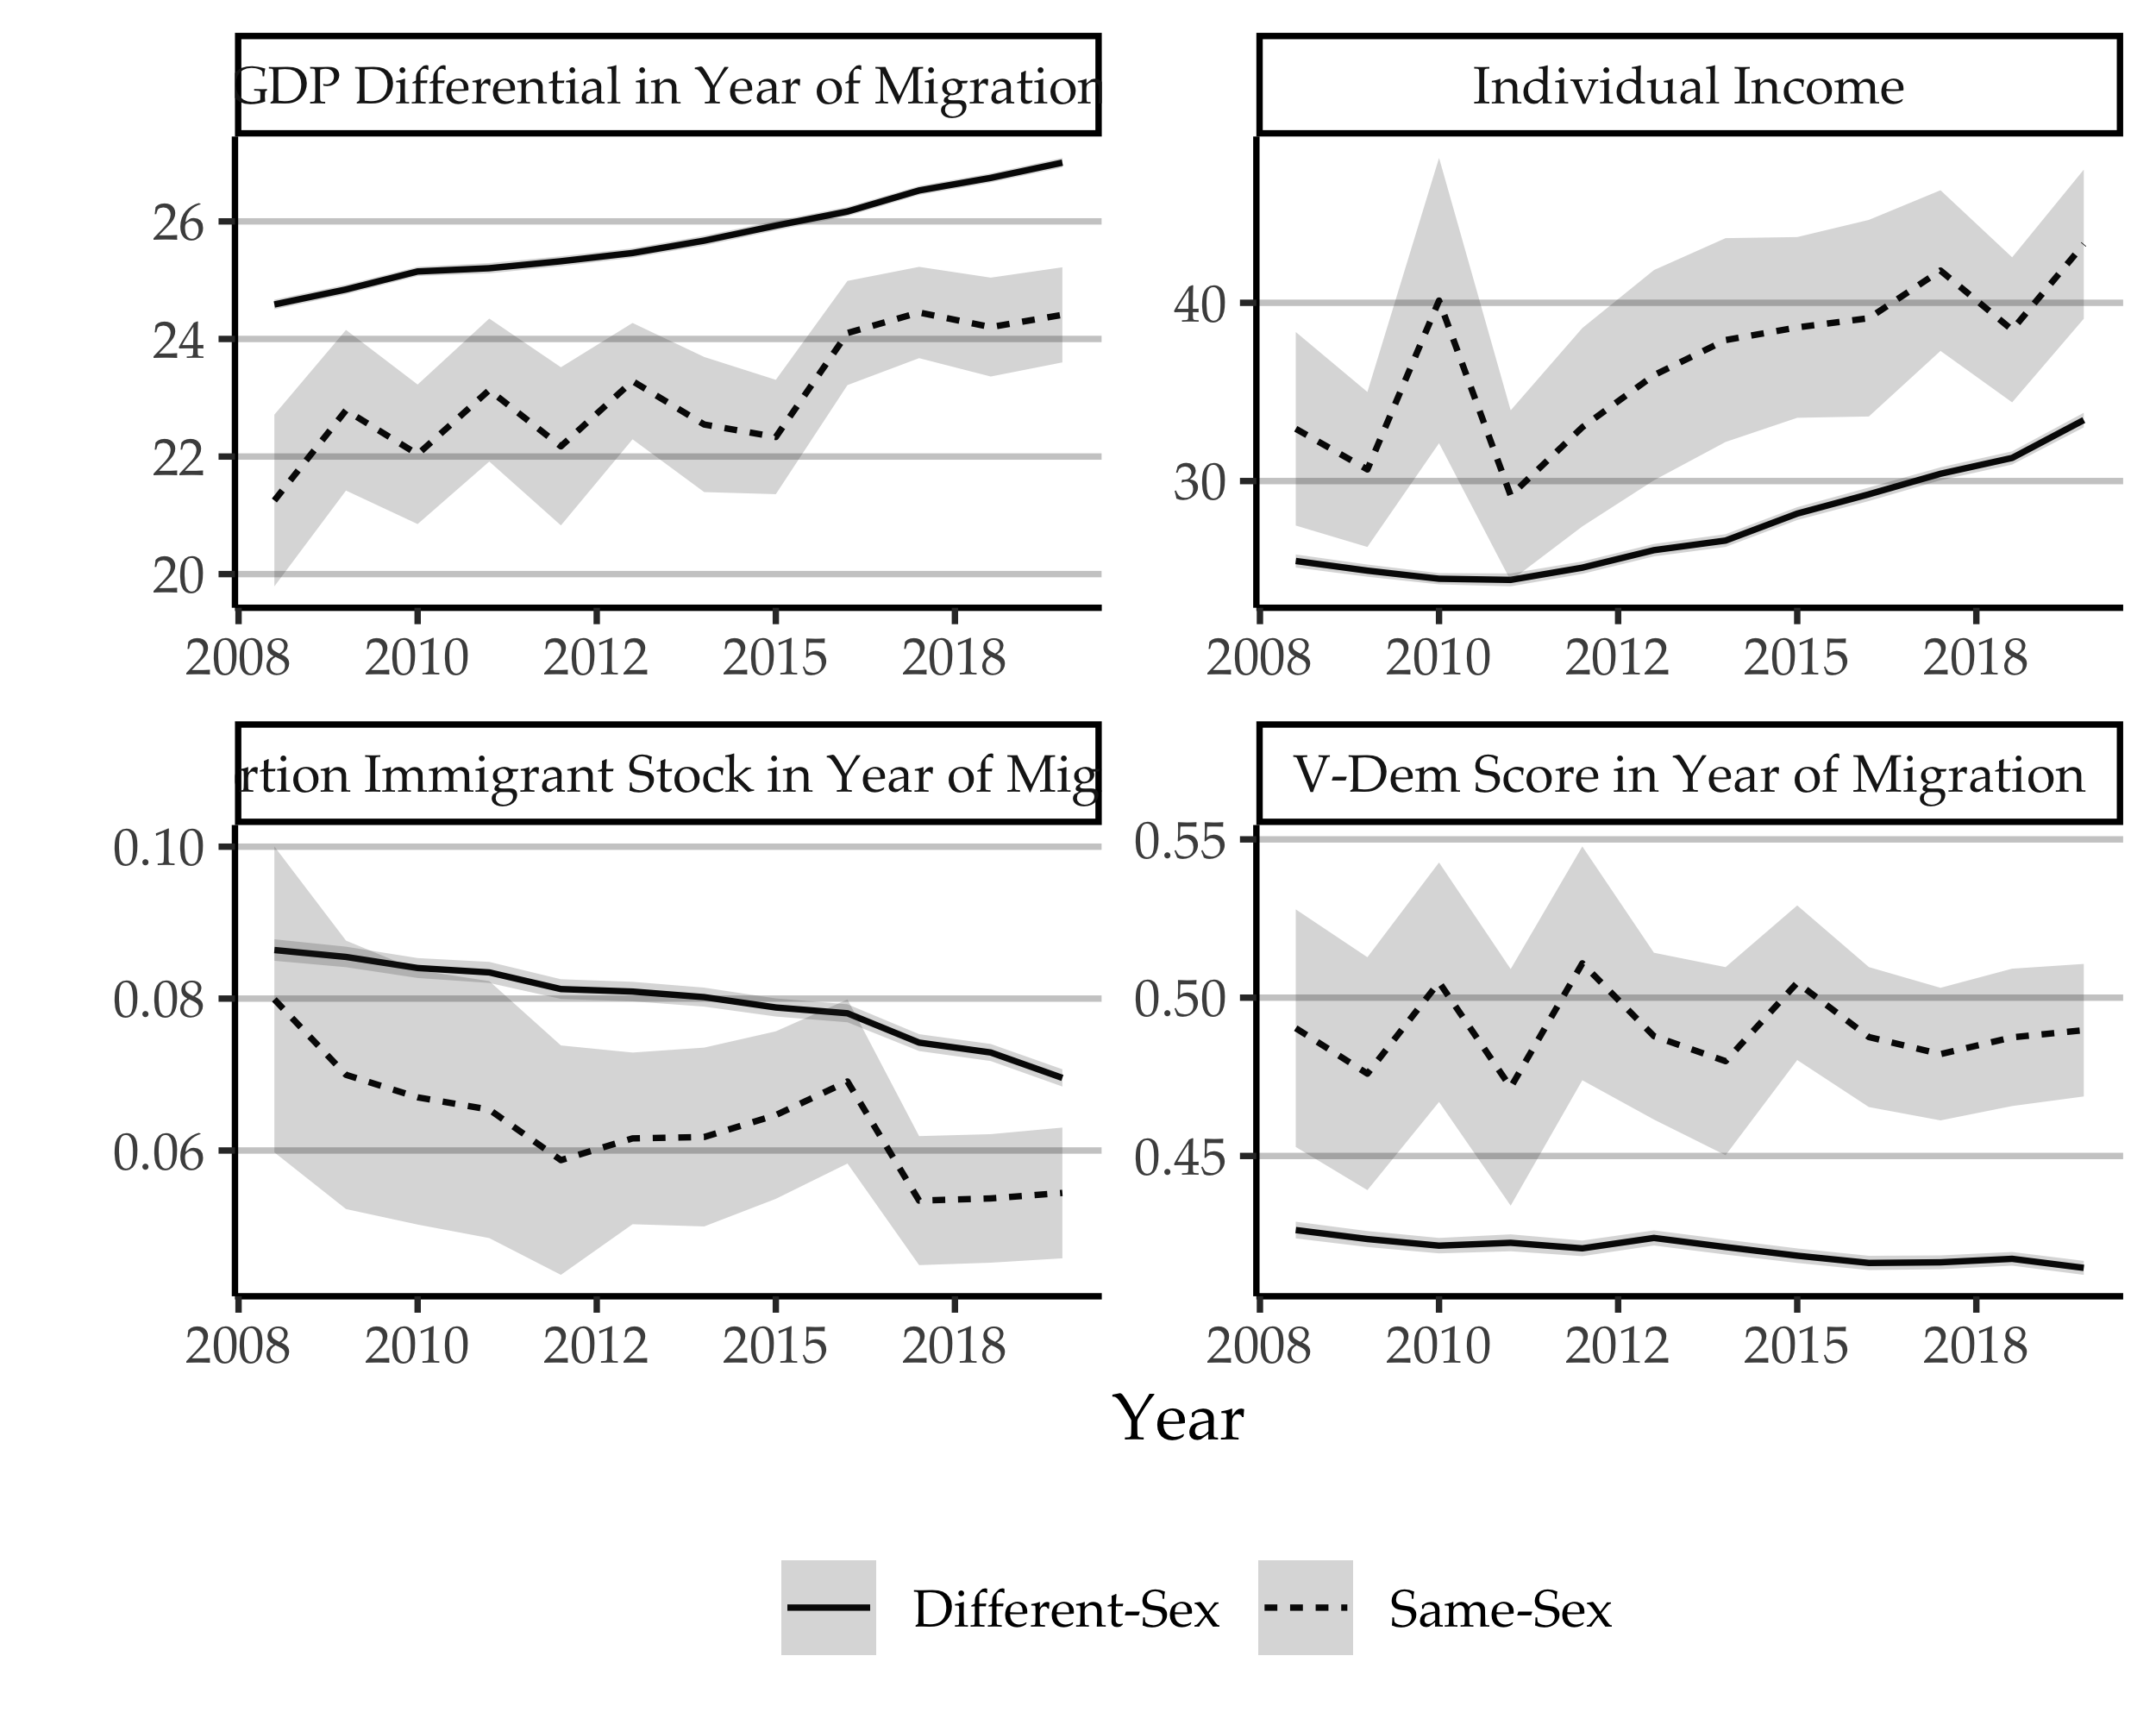
\includegraphics{ssimm_pres_files/figure-beamer/desc-1.pdf}
\end{frame}

\begin{frame}{Descriptive statistics}
\protect\hypertarget{descriptive-statistics-1}{}
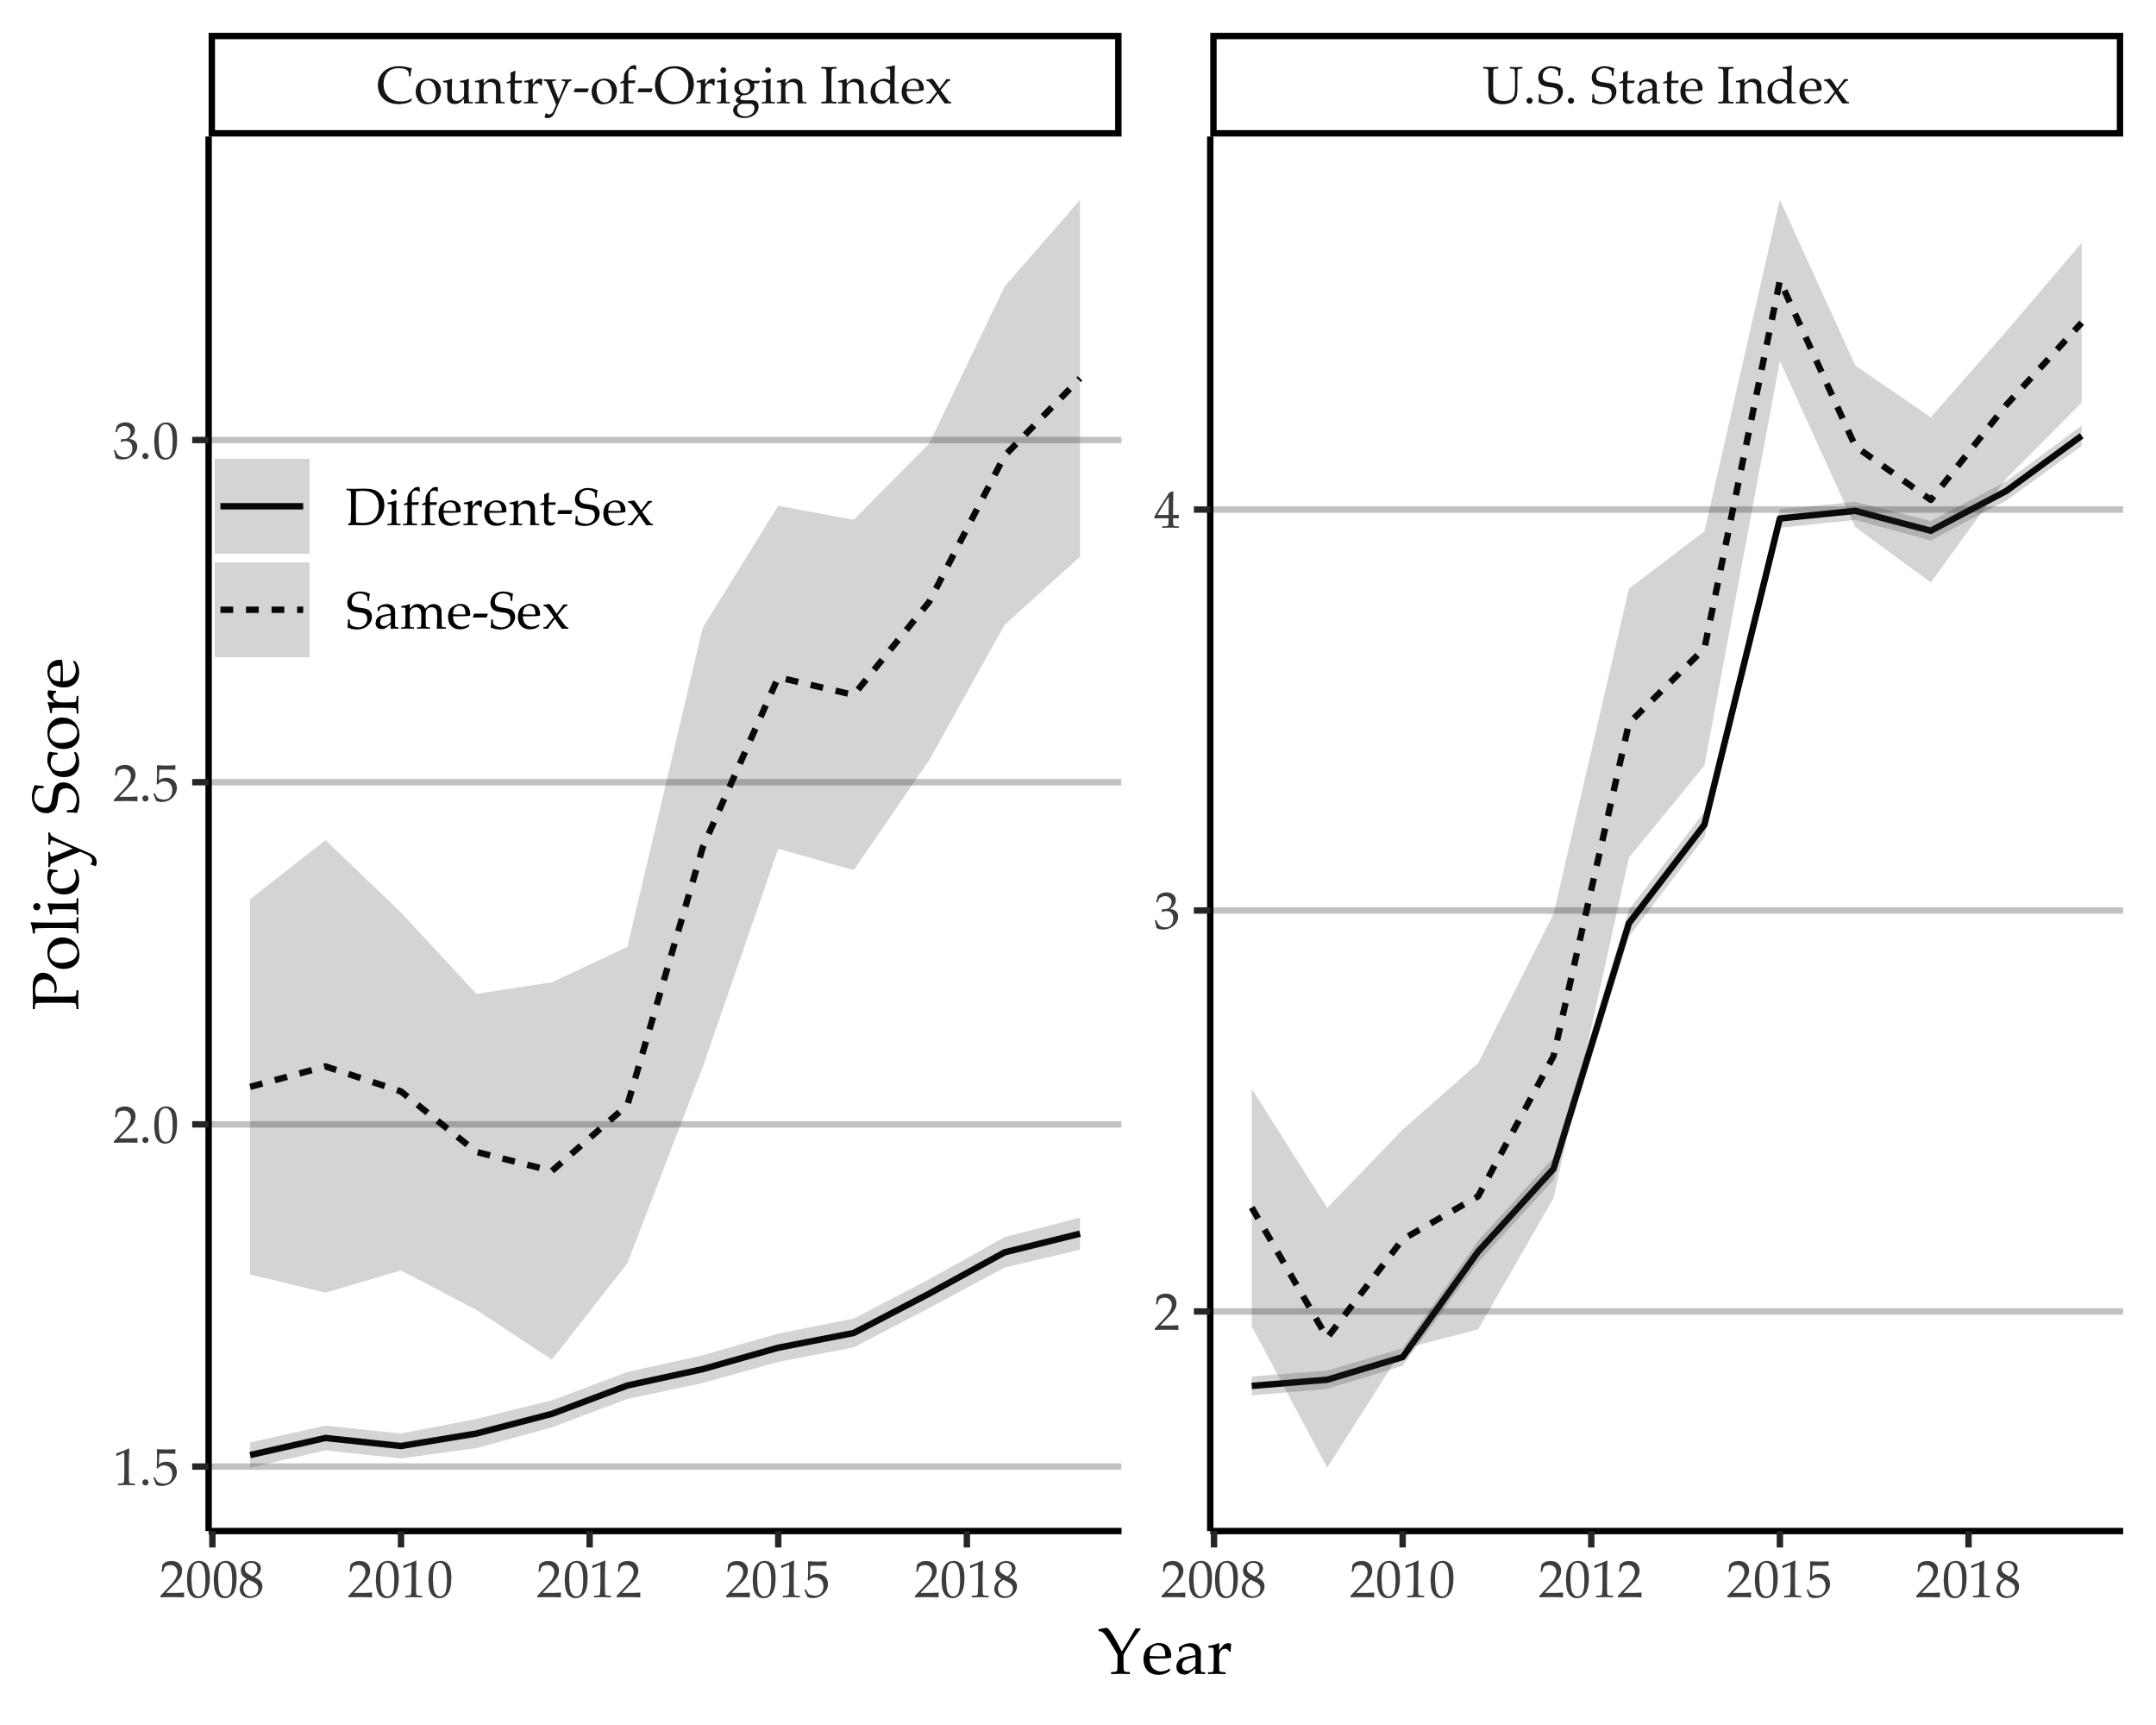
\includegraphics{ssimm_pres_files/figure-beamer/policy-desc-1.pdf}
\end{frame}

\begin{frame}{Descriptive statistics}
\protect\hypertarget{descriptive-statistics-2}{}
\begin{table}

\caption{\label{tab:country-tab}Sending countries ranked by proportion immigrant couples with same-sex partners}
\centering
\fontsize{9}{11}\selectfont
\begin{tabular}[t]{lllr}
\toprule
Rank & Country of origin & Proportion same-sex & Mean policy score\\
\midrule
1 & Belgium & 2.98 \% & 6.30\\
2 & Australia & 2.72 \% & 5.08\\
3 & Netherlands & 2.60 \% & 9.24\\
4 & Malaysia & 2.55 \% & -0.90\\
5 & Bahamas & 2.43 \% & 0.85\\
6 & Mongolia & 2.41 \% & 2.26\\
7 & Zimbabwe & 2.38 \% & -0.96\\
8 & New Zealand & 2.37 \% & 6.99\\
9 & Finland & 2.35 \% & 5.67\\
10 & Singapore & 2.34 \% & 0.10\\
\bottomrule
\multicolumn{4}{l}{\rule{0pt}{1em}\textit{Source:} American Community Survey 2008-2019. Authors' calculations.}\\
\end{tabular}
\end{table}
\end{frame}

\begin{frame}{Descriptive statistics}
\protect\hypertarget{descriptive-statistics-3}{}
\begin{table}

\caption{\label{tab:state-tab}States ranked by proportion immigrant couples with same-sex partners}
\centering
\fontsize{9}{11}\selectfont
\begin{tabular}[t]{lllr}
\toprule
Rank & State & Proportion same-sex & Mean policy score\\
\midrule
1 & Vermont & 2.10 \% & 5.26\\
2 & Maine & 1.51 \% & 4.86\\
3 & Montana & 1.47 \% & 0.94\\
4 & Missouri & 1.11 \% & 1.96\\
5 & Massachusetts & 1.10 \% & 4.80\\
6 & New York & 1.08 \% & 4.90\\
7 & Florida & 0.99 \% & 1.00\\
8 & New Hampshire & 0.95 \% & 4.40\\
9 & Minnesota & 0.92 \% & 4.67\\
10 & New Mexico & 0.92 \% & 4.80\\
\bottomrule
\multicolumn{4}{l}{\rule{0pt}{1em}\textit{Source:} American Community Survey 2008-2019. Authors' calculations.}\\
\end{tabular}
\end{table}
\end{frame}

\begin{frame}{Model Results: Country-of-Origin Effects}
\protect\hypertarget{model-results-country-of-origin-effects}{}
\begin{table}[!htbp] \centering 
  \caption{Percent of immigrants in same-sex couples by year of immigration and country of origin.} 
  \label{tab:country-props} 
\tiny 
\begin{tabular}{@{\extracolsep{3pt}}lccccc} 
\\[-1.8ex]\hline 
\hline \\[-1.8ex] 
 & \multicolumn{5}{c}{\textit{Dependent variable:}} \\ 
\cline{2-6} 
\\[-1.8ex] & \multicolumn{5}{c}{Percent in same-sex couples by country-year} \\ 
\\[-1.8ex] & (1) & (2) & (3) & (4) & (5)\\ 
\hline \\[-1.8ex] 
 Country LGBT policy score & 0.037$^{***}$ & 0.036$^{***}$ & 0.021$^{***}$ & $-$0.006 & $-$0.015$^{*}$ \\ 
  & (0.004) & (0.005) & (0.005) & (0.005) & (0.006) \\ 
  & & & & & \\ 
 Polity5 democracy score &  & 0.003 & $-$0.002 & 0.001 & 0.001 \\ 
  &  & (0.002) & (0.002) & (0.002) & (0.002) \\ 
  & & & & & \\ 
 Post-2013 &  &  &  & 0.310$^{***}$ & 0.250$^{***}$ \\ 
  &  &  &  & (0.022) & (0.034) \\ 
  & & & & & \\ 
 Country score × Post-2013 &  &  &  &  & 0.026$^{**}$ \\ 
  &  &  &  &  & (0.010) \\ 
  & & & & & \\ 
\hline \\[-1.8ex] 
Country controls? & no & yes & yes & yes & yes \\ 
Country FEs? & no & no & yes & yes & yes \\ 
Observations & 30,078 & 30,078 & 30,078 & 30,078 & 30,078 \\ 
\hline 
\hline \\[-1.8ex] 
\multicolumn{6}{l}{Note: †p<0.1; *p<0.05; **p<0.01; ***p<0.001} \\ 
\end{tabular} 
\end{table}
\end{frame}

\begin{frame}{Model Results: State Effects}
\protect\hypertarget{model-results-state-effects}{}
\begin{table}[!htbp] \centering 
  \caption{Percent same-sex in by country of origin, U.S. state, and survey year.} 
  \label{tab:state-props} 
\tiny 
\begin{tabular}{@{\extracolsep{3pt}}lcccccc} 
\\[-1.8ex]\hline 
\hline \\[-1.8ex] 
 & \multicolumn{6}{c}{\textit{Dependent variable:}} \\ 
\cline{2-7} 
\\[-1.8ex] & \multicolumn{6}{c}{Percent in same-sex couples by state-country-year} \\ 
\\[-1.8ex] & (1) & (2) & (3) & (4) & (5) & (6)\\ 
\hline \\[-1.8ex] 
 State LGBT policy score & 0.063$^{***}$ & 0.058$^{***}$ & 0.026 & 0.015 & $-$0.002 & 0.002 \\ 
  & (0.016) & (0.016) & (0.035) & (0.035) & (0.035) & (0.036) \\ 
  & & & & & & \\ 
 Country LGBT policy score &  & 0.078$^{***}$ & 0.071$^{***}$ & 0.120$^{**}$ & 0.090$^{*}$ & $-$0.007 \\ 
  &  & (0.009) & (0.009) & (0.038) & (0.039) & (0.047) \\ 
  & & & & & & \\ 
 Post-2013 &  &  &  &  & 0.240$^{***}$ & 0.110 \\ 
  &  &  &  &  & (0.068) & (0.077) \\ 
  & & & & & & \\ 
 Country score × Post-2013 &  &  &  &  &  & 0.075$^{***}$ \\ 
  &  &  &  &  &  & (0.021) \\ 
  & & & & & & \\ 
\hline \\[-1.8ex] 
State controls and FEs? & no & no & yes & yes & yes & yes \\ 
Country controls and FEs? & no & no & no & yes & yes & yes \\ 
Observations & 35,636 & 35,636 & 35,636 & 35,636 & 35,636 & 35,636 \\ 
\hline 
\hline \\[-1.8ex] 
\multicolumn{7}{l}{Note: †p<0.1; *p<0.05; **p<0.01; ***p<0.001} \\ 
\end{tabular} 
\end{table}
\end{frame}

\begin{frame}{Model Results: Individual Analysis}
\protect\hypertarget{model-results-individual-analysis}{}
\begin{table}[!htbp] \centering 
  \caption{Individual ordered logit analysis of three-category state policy score.} 
  \label{tab:ord} 
\tiny 
\begin{tabular}{@{\extracolsep{3pt}}lccc} 
\\[-1.8ex]\hline 
\hline \\[-1.8ex] 
 & \multicolumn{3}{c}{\textit{Dependent variable:}} \\ 
\cline{2-4} 
\\[-1.8ex] & \multicolumn{3}{c}{Binned state LGBT policy score} \\ 
\\[-1.8ex] & (1) & (2) & (3)\\ 
\hline \\[-1.8ex] 
 Same-sex & 0.190$^{***}$ & 0.110$^{**}$ & 21.000$^{***}$ \\ 
  & (0.025) & (0.035) & (0.0004) \\ 
  & & & \\ 
 Country LGBT policy score &  & $-$0.044$^{***}$ & $-$0.030$^{***}$ \\ 
  &  & (0.003) & (0.003) \\ 
  & & & \\ 
 Same-sex × country score &  & 0.041$^{***}$ & 0.051$^{***}$ \\ 
  &  & (0.009) & (0.009) \\ 
  & & & \\ 
\hline \\[-1.8ex] 
Survey year FEs? & yes & yes & yes \\ 
Individual controls? & no & no & yes \\ 
Observations & 107,500 & 107,500 & 107,500 \\ 
\hline 
\hline \\[-1.8ex] 
\multicolumn{4}{l}{Note: †p<0.1; *p<0.05; **p<0.01; ***p<0.001} \\ 
\end{tabular} 
\end{table}
\end{frame}

\begin{frame}{Model Results: Individual Analysis}
\protect\hypertarget{model-results-individual-analysis-1}{}
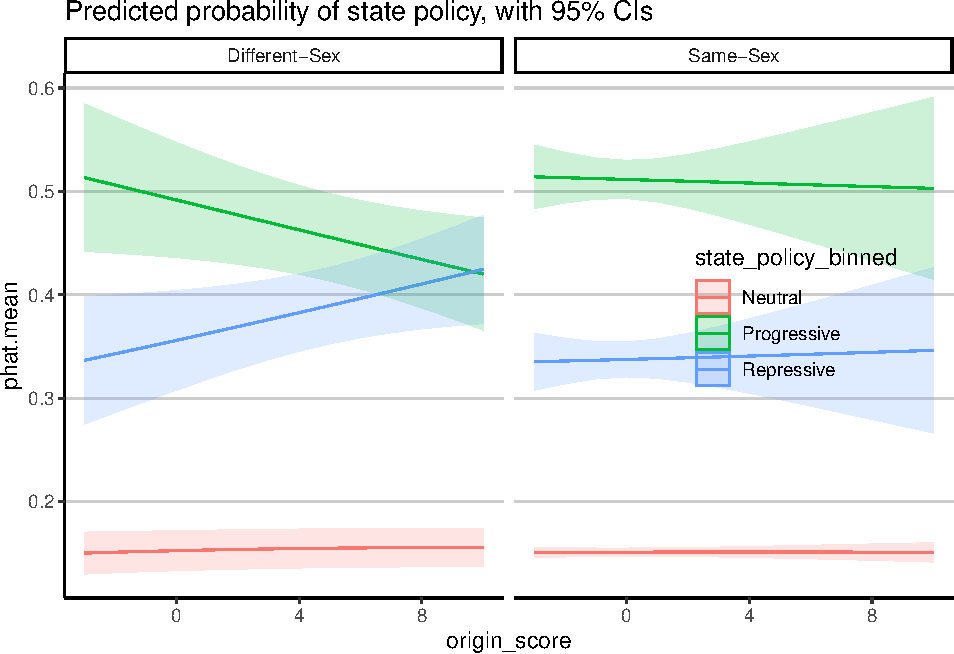
\includegraphics{ssimm_pres_files/figure-beamer/sim-1.pdf}
\end{frame}

\hypertarget{discussion}{%
\section{Discussion}\label{discussion}}

\begin{frame}{Discussion}
\protect\hypertarget{discussion-1}{}
\begin{itemize}
\tightlist
\item
  Immigrants in same-sex couples have higher income, occupational
  prestige, and education than those in different-sex couples
\item
  Progressive countries send higher proportions of immigrants in
  same-sex couples

  \begin{itemize}
  \tightlist
  \item
    Counter to existing, mostly qualitative scholarship of queer
    migration
  \end{itemize}
\item
  Mixed evidence that immigrants in same-sex couples reside in more
  progressive U.S. states
\item
  Policies not explicitly related to migration may shape migration flows

  \begin{itemize}
  \tightlist
  \item
    Importance of migration scholars studying the state's governance of
    identity
  \item
    Need to move beyond the traditional economic and network
    explanations of migration
  \end{itemize}
\end{itemize}
\end{frame}

\hypertarget{section}{%
\section{}\label{section}}

\begin{frame}{}
\begin{center}
  \huge{\textcolor{uclablue}{Thank You}}
\end{center}

\begin{itemize}
\tightlist
\item
  Nathan I. Hoffmann (\textcolor{uclablue}{nathanihoff\@ucla.edu})
\item
  Kristopher Velasco (\textcolor{uclablue}{krisvelasco\@utexas.edu})
\end{itemize}
\end{frame}

\end{document}
